\chapter{Analysis and methodology}
\label{ana-meth}

This chapter presents all the implemented load forecasting models.
The choice of each model is justified, and the architecture of each model is described with sufficient detail for it to be implemented.

\section{Investigated models and methods}

A time series forecasting model can generally be structured as a model that takes as input one or more matrices of historical and/or forecast data, and produces an output matrix of predictions.
This structure is rather generic, and there are many models that can fulfil this requirement.
However, for this thesis, only a handful of models have been selected for evaluation.
Each model will be discussed briefly here, to provide the reader with a high-level overview, and then each model will be discussed in detail under its own heading in the following pages.

The seasonal autoregressive integrated moving average with exogenous factors (SARIMAX) model is an extension of the well known ARIMA \cite{Box1970} model which takes into account seasonal patterns and exogenous data.
It has been around unchanged for decades and is used as a baseline for forecasting performance.

Sequence to sequence recurrent neural networks with long short-term memory cells gained notoriety in the field of neural machine translation in 2014 for achieving state of the art results with minimal tuning of the model \cite{sutskever2014sequence}.
The structure of this model is a natural fit for time series forecasting - neural machine translation maps one sequences of words (vectors) to another, just as a time series forecasting system maps a sequence of historical observations (vectors) to a sequence of predicted observations (also vectors).
The simplicity and out-of-the-box performance of this model is extremely appealing.

The transformer neural network model was published in 2017, and produced state of the art results in neural machine translation using a fully attention-based architecture.
This model is attractive because it may overcome the tendency for recurrent neural networks to ``forget" data from early in the input sequence, while also having the ability to consider multiple information sub-spaces in the input.

The universal transformer model, published in July 2018, is a variant of the transformer, and claims to out-perform the transformer on algorithmic tasks.
This model is included to assess its performance compared to the transformer.

Additionally, a similar profile selection method was developed to provide the models with relevant input data.

\section{Seasonal autoregressive integrated moving average with exogenous factors}

The seasonal autoregressive integrated moving average with exogenous factors (SARIMAX) model is comprised of autoregressive (AR) and moving average (MA) terms.
These will be described first and then used to build the SARIMAX model.

Consider a univariate time series $\vx \in \mathbb{R}^{T}$, being drawn from some underlying process, with scalar elements $x_{t-1}, ..., x_{0}$. 
An autoregressive model predicts the next element of the series by
\begin{equation}
x_{t} = \alpha_{1}x_{t-1} + \alpha_{2}x_{t-2} + \ldots + \alpha_{p}x_{t-p} + \epsilon_{t} = \epsilon_{t} + \sum_{i=1}^{p}\alpha_{i}x_{t-i}
\end{equation}
where $p$ is the order of the AR model, $\alpha$ are the parameters of the model, and $\epsilon_{t}$ is a random normally distributed error with zero mean and variance $\sigma^2$. 

A moving average model predicts the next element of the series by
\begin{equation}
x_{t} = \theta_{1}\epsilon_{t-1} + \theta_{2}\epsilon_{t-2} + \ldots + \theta_{q}\epsilon_{t-q} + \epsilon_{t} = \epsilon_{t} + \sum_{i=1}^{q}\theta_{i}\epsilon_{t-i}
\end{equation}
where $q$ is the order of the MA model, $\theta$ are the parameters of the model, and $\epsilon_{t}$ is, again, a random normally distributed error with zero mean and variance $\sigma^2$.

The AR and MA models can be combined to form an ARMA model, given by 
\begin{equation}
x_{t} = \epsilon_{t} + \sum_{i=1}^{q}\theta_{i}\epsilon_{t-i} + \sum_{i=1}^{p}\alpha_{i}x_{t-i}
\end{equation}

An ARMA model requires the time series, $\vx$, being forecast to come from a weakly stationary process.
That is, the mean and autocovariance of the the process do not change with time.
The ARIMA model is an extension to the ARMA model that can be applied when non-stationarity is exhibited by the underlying process.
ARIMA applies differencing to the time series to produce $\hat{\vx}$, and then applies the ARMA model.
This differencing is applied such that $\hat{x}_{t} = x_{t} - x_{t-1}$ and is repeated $d$ times.
Differencing can sometimes be sufficient to make a series stationary, such that it is appropriate for forecasting with an ARMA model.

In order to concisely articulate the ARIMA model, the following notation will be used.
Note that this notation overrides that defined in the \nameref{section:Nomenclature} section.
\begin{itemize}
	\item The backward shift operator, defined by $\textbf{B}^{m}x_{t} = x_{t-m}$. 
	\item The difference operator, defined by $\nabla_{s} X_{t} = x_{t} - x_{t-s} = (1 - \textbf{B}^{s})x_{t}$. 
	\item The parameter functions $\alpha_{p}(\textbf{B}) = 1 - \alpha_{1}\textbf{B} - \ldots - \alpha_{p}\textbf{B}^p$ and $\theta_{q}(\textbf{B}) = 1 + \theta_{1}\textbf{B} + \ldots + \theta_{q}\textbf{B}^q$.
\end{itemize}
Note that the difference operator can be raised to a power to allow repeated differencing, such that $\nabla_{s}^{u} X_{t} = [(1 - \textbf{B}^{s})^{u}]x_{t}$.
Using this notation, the ARIMA model can be represented by the following expression
\begin{equation}
\alpha_{p}(\textbf{B})(\nabla_{1}^{d}x_{t}) = \theta_{q}(\textbf{B})\epsilon_{t}
\end{equation}
This is identical to an ARMA model, except that $x_{t}$ has been replaced with a  version of itself, $\nabla_{1}^{d}x_{t}$, that has been differenced $d$ times.
The above model is denoted ARIMA($p,d,q$).

Differencing with a lag of one is not always sufficient to make the series stationary even when performed multiple ($d$) times.
A further extension of the ARIMA model is the seasonal ARIMA (SARIMA) model, which takes into account seasonal patterns which require differencing with a lag greater than one, such as daily, weekly, and yearly seasonalities commonly found in electrical load time series.
\\
Denoted ARIMA$(p,d,q)\times(P,D,Q)s$, a SARIMA model can be represented as the following
\begin{equation}
\alpha_{p}(\textbf{B})A_{P}(\textbf{B}^{s})(\nabla_{1}^{d}\nabla_{s}^{D}x_{t}) = \theta_{q}(\textbf{B})\Theta_{Q}(\textbf{B}^{s})\epsilon_{t}
\end{equation}
where $(p,d,q)$ are the parameters of the non-seasonal ARIMA component, $(P,Q,D)s$ are the parameters of the seasonal component, $A_{P}(\textbf{B}^{s})$ and $\Theta_{Q}(\textbf{B}^{s})$ are defined similarly to $\alpha_{p}(\textbf{B})$ and $\theta_{q}(\textbf{B})$, and $s$ is the number of periods over which the seasonality occurs (e.g. $s=7$ for weekly seasonality if the data is daily).

The SARIMA model can be further extended to a SARIMA with exogenous variables (SARIMAX) model.
Given a vector of exogenous inputs $\vz \in \mathbb{R}^{n}$ corresponding to the exogenous inputs at time $t$, the SARIMAX model gives the next element of the series by
\begin{gather}	
\alpha_{p}(\textbf{B})A_{P}(\textbf{B}^{s})(\nabla_{1}^{d}\nabla_{s}^{D}u_{t}) = \theta_{q}(\textbf{B})\Theta_{Q}(\textbf{B}^{s})\epsilon_{t} \\	
x_{t} = u_{t} + \sum_{i=1}^{n}\beta_{i}z_{i}
\end{gather}
where $\beta_{1} \ldots \beta_{n}$ are a set of model parameters.

\subsection{Implementation}
A SARIMAX model was implemented using the python statsmodels package.


\section{Neural networks - a primer}
Neural networks will be described in a general sense here prior to discussion of the specific neural network architectures in the following sections.
This section intends to establish the fundamental concepts that are applied when developing neural network models.

An artificial neural network (ANN) is a method for computation based loosely on biological brains \citep{negnevitsky2005artificial}.
An ANN is simply a function approximator; given a function $f^*(\vx)$, an ANN defines an approximation function $f(\vx; \vtheta)$ where $\vtheta$ is a (usually learned) set of parameters that lead to the best approximation of $f^*$ \citep{Goodfellow-et-al-2016}. 
Generally, ANNs are formed by combining many fundamental sub-functions in a graph-like manner. 
A simple example is the multilayer perceptron.
Consider a single perceptron, shown in figure \ref{fig:single-perceptron}.
This single perceptron simply takes the weighted sum of all inputs plus a bias and applies an activation function, usually differentiable and highly non-linear, to produce an output $y$.
A multilayer perceptron is formed by structuring individual perceptrons in layers and cascading them so that the outputs of the perceptrons in one layer are the inputs to the perceptrons in the next layer, as shown in figure \ref{fig:mlayer-perceptron} where the lines indicate connections from the output of one perception to the input of the next.
The weights $w$ are mapped to elements in the parameter vector $\vtheta$.

The hidden layer can be repeated any number of times, allowing the neural network to be written in the form $f(\vx) = f^n(f^{\ldots}(f^1(\vx)))$.
This is a feedforward neural network, and is the only type of neural network this thesis will consider.
In the case of recurrent neural networks discussed later in this thesis, where the outputs of sub-functions in the network form cycles, the network is unrolled to form a feedforward network.

\begin{figure}[htbp]
	\centering
	\subfigure[A single perceptron.]{
	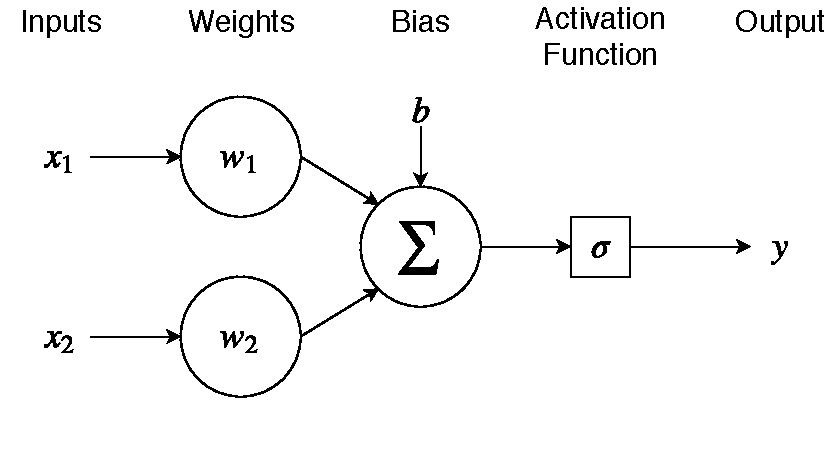
\includegraphics[width=.45\textwidth]{images/perceptron.pdf}
	\label{fig:single-perceptron}}
	%\vfil
	\quad\quad
	\subfigure[A multi-layer perceptron, with each circle representing a single perceptron.]{
	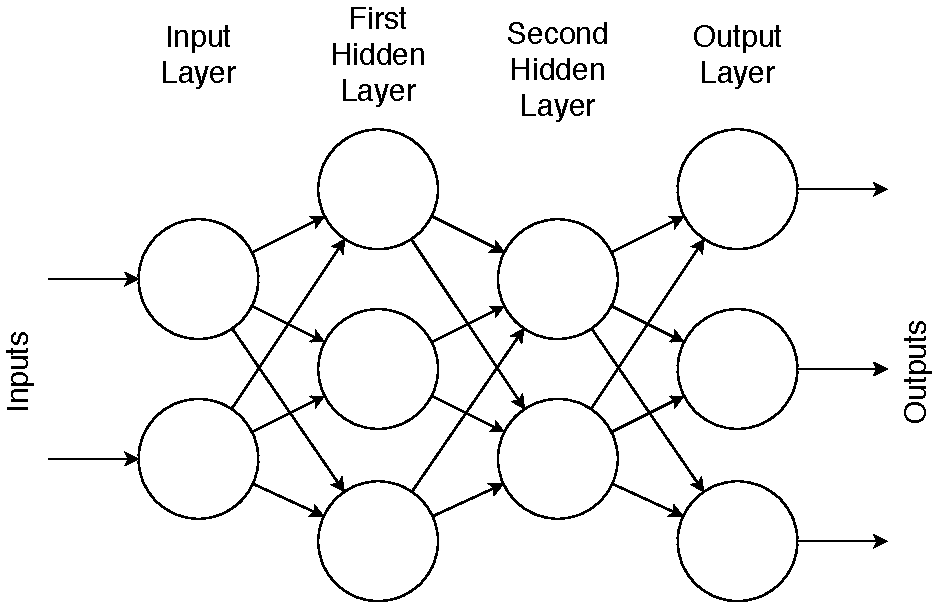
\includegraphics[width=.45\textwidth]{images/MLP.pdf}
	\label{fig:mlayer-perceptron}}
	\caption{A multilayer perceptron is comprised of multiple individual perceptrons.}
	\label{fig:simple-ann}
\end{figure}

The set of parameters $\vtheta$ is usually learned, or trained, by stochastic gradient descent \citep{Bottou2011} or a variant thereof.
Consider an ANN producing an approximated output $\hat{\vy} = f(\vx; \vtheta)$ and a cost function $J(\vy, \hat{\vy}) = J(\vy, \vx, \vtheta)$, with  $J$ being a differentiable function of its inputs, $\vy$ being the correct output of $f^*$, and $\vtheta$ being randomly initialized.
The cost function produces a scalar describing the error between $\vy$ and $\hat{\vy}$.
A common example of this is sum squared error, where $J(\vy, \hat{\vy}) = \sum_{n=o}^{i}(|\vy_n - \hat{\vy}_n|^2)$.
The gradient of $J$ with respect to the parameters is given by $\nabla_{\vtheta}J(\vy, \vx, \vtheta)$ and indicates the direction in which to move $\vtheta$ in order to increase $J$.
By iteratively applying equation \ref{gradient_descent}, where $\epsilon$ is a scalar constant referred to as the learning rate, the value of $\vtheta$ will be modified such that $J(\vy, \vx, \vtheta)$ is minimized - thus maximizing the approximation accuracy of $f$ as measured by $J$.
The action of applying equation \ref{gradient_descent} a single time is commonly referred to as taking a single training step, operation or iteration.

\begin{equation} \label{gradient_descent}
\vtheta = \vtheta - \epsilon \nabla_{\vtheta}J(\vy, \vx, \vtheta)
\end{equation}

In stochastic gradient descent, $\vx$ and $\vy$ are a randomly selected pair from the training set and so over many training iterations the entire training set will be approximately uniformly sampled.
Typically, though, mini-batch gradient descent is used rather than stochastic gradient descent, whereby the training step is batched -- multiple pairs of $\vx$ and $\vy$ are used to average the loss in parallel before performing an update on the weight vector.
The number of pairs of $\vx$ and $\vy$ per batch is commonly referred to as the batch size.
Mini-batch gradient descent is generally able to leverage parallel computation features of modern microprocessors to make it vastly faster than calculating $J$ multiple times and taking the average.

Whether the loss minimization process lands on a global or local minimum is dependant on the function $J$ and the specifics of the gradient descent implementation.
Using a smaller batch size will introduce noise into the loss function, making it more likely for the optimization process to escape local minima, while using a larger learning rate might allow the training operation to ``jump" out of local minima.
Of course, both of these have downsides too -- arguments for larger batch size and smaller learning rate can also be made. 
Overall, the training process is complex and nuanced.
The training processes used in this thesis are discussed in section \ref{train-reg}.


\section{Recurrent neural network}
The recurrent neural network (RNN) architecture was introduced by \citet{Rumelhart1986} in 1986.
Over the past five years RNN-based neural network models have achieved state of the art performance -- though in many cases have since been outperformed by more obscure models -- in speech recognition \cite{Chiu2017}, neural machine translation \cite{luong2015effective}, image captioning \cite{yao2017boosting}, and time series classification \cite{Karim2018}.
Over this same time span RNN-based neural networks have been used to forecast electrical load at the household-level \cite{Kong2017}\cite{Shi2018}, building level \cite{Zheng2017a}, feeder-level \cite{Bedi2018}, and city/state level \cite{Narayan2017}\cite{Din2017}.
RNN-based models appear to offer the ability to forecast load with minimal preprocessing of the input data and so may be a very attractive option for practical load forecasting systems.

\subsection{Generic recurrent neural network}
RNNs operate on sequences of data by applying an identical function $f$ to every element of the sequence to produce a sequence of state vectors $\mH = [\vh_1 \, \ldots \, \vh_P]$.
$f$ takes as input both the output of the function at the previous point in the sequence, and the current element of the input sequence $\mX = [\vx_1 \, \ldots \, \vx_P]$.
An RNN can be unfolded to represent it as a traditional feedforward neural network with no recurrence.
A generic RNN is shown in figure \ref{fig:basic_rnn}.

At each point $t$ in the sequence $\vh_t$ is taken as the output.
$\vh_t$ can be projected to the required output dimension - for example by equation \ref{dense_layer}, but any method can be used.
An output dimension of 1 is typical for univariate load forecasting.

RNNs can be extended to multiple layers, with a two-layer RNN illustrated in figure \ref{fig:multilayer_rnn}.
Each layer implements its own function, with layer $n$ implementing function $f^n$ and producing output $\vh^n$.
For layers after the first layer, instead of taking an $\vx$ vector as input they take the state vector from the previous layer.
There can be an arbitrary number of layers.
A multi-layer RNN can in fact be thought of as a generalization of a single-layer, where the function $f$ is simply comprised of multiple sub-functions.

\begin{figure}[htbp]
	\centering
	\subfigure[A generic recurrent neural network.]{
		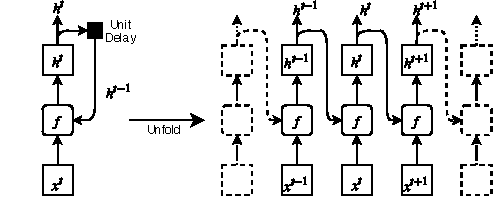
\includegraphics[width=.5\textwidth]{images/basic_rnn.pdf}
		\label{fig:basic_rnn}}
	%\vfil
	\quad\quad
	\subfigure[A two-layer recurrent neural network.]{
		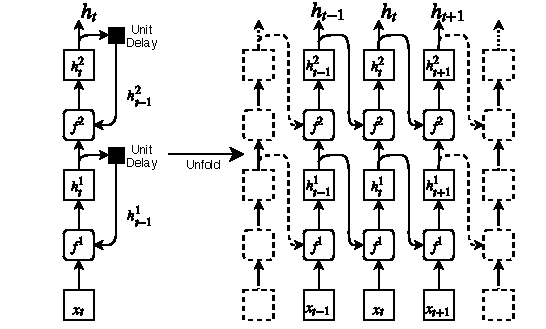
\includegraphics[width=.5\textwidth]{images/multilayer_rnn.pdf}
		\label{fig:multilayer_rnn}}
	\caption{Recurrent neural networks in single- and multi-layer configurations, with both recurrent and unrolled feedforward representations shown. }
	\label{fig:rnn}
\end{figure}


\subsection{Long short-term memory}
RNNs are prone to issues with vanishing and exploding gradients \cite{Goodfellow-et-al-2016}, which can be addressed through the use of a long short-term memory (LSTM) \cite{hochreiter1997long} cell as the function in the RNN.
An LSTM cell is able to selectively add and remove elements from the state vector as it passes through the cell.
LSTM cells have been demonstrated to outperform simpler functions in a variety of tasks when employed as the RNN function \cite{Chung2014}\cite{jozefowicz2015empirical}\cite{le2015simple}.
The LSTM cell extends the standard RNN model by separating the cell output $\vc_t$ from the cell state $\vh_t$, shown in figure \ref{fig:LSTM_cell}, and its multi-layer configuration shown in figure \ref{fig:LSTM_multilayer}.
The LSTM cell is described by the following equations
\begin{align}
\vf_t &= \sigma(\mW_{f} \vx_t + \mU_{f} \vh_{t-1} + \vb_f) \label{eq:forget_lstm}\\
\vi_t &= \sigma(\mW_{i} \vx_t + \mU_{i} \vh_{t-1} + \vb_i) \\
\vo_t &= \sigma(\mW_{o} \vx_t + \mU_{o} \vh_{t-1} + \vb_o) \\
\hat{\vc}_t &= \text{tanh}(\mW_{c} \vx_t + \mU_{c} \vh_{t-1} + \vb_c) \\
\vc_t &= \vf_t \circ \vc_{t-1} + \vi_t \circ \hat{\vc}_t \\
\vh_t &= \vo_t \circ \text{tanh}(\vc_t) \label{eq:cell_state_lstm}
\end{align}

where 
\begin{itemize}
	\item $\circ$ denotes element-wise multiplication;
	\item the input vector $\vx_t \in \mathbb{R}^{N}$;
	\item the cell output vector $\vh_t \in \mathbb{R}^{d}$ ($d$ is the hidden dimension of the model);
	\item the cell state vector $\vc_t \in \mathbb{R}^{d}$;
	\item  the forget gate vector $\vf_t \in \mathbb{R}^{d}$;
	\item the input gate vector $\vi_t \in \mathbb{R}^{d}$;
	\item the output gate vector $\vo_t \in \mathbb{R}^{d}$;
	\item the cell candidate vector $\hat{\vc}_t \in \mathbb{R}^{d}$;
	\item the learned cell state weight matrices $\mU \in \mathbb{R}^{d \times N}$;
	\item the learned input weight matrices $\mW \in \mathbb{R}^{d \times d}$;
	\item the learned bias vectors $\vb \in \mathbb{R}^{d}$; and
	\item $\sigma(\vy) = \frac{1}{1 + e^{-\vy}}$ represents the sigmoid function.
\end{itemize}

At first glance equations \ref{eq:forget_lstm} through \ref{eq:cell_state_lstm} may come across as esoteric, but they are in fact highly intuitive when studied alongside figure \ref{fig:LSTM}.
There are three primary sub-sections within the LSTM cell, discussed in the three following paragraphs.
Note that the use of two weight matrices ($\mW$ and $\mU$) in the LSTM equations is equivalent to concatenating $\vx$ and $\vh$ and using a single weight matrix - keeping consistency with figure \ref{fig:LSTM}.

\begin{figure}[htbp]
	\centering
	\subfigure[A long short-term memory cell.]{
		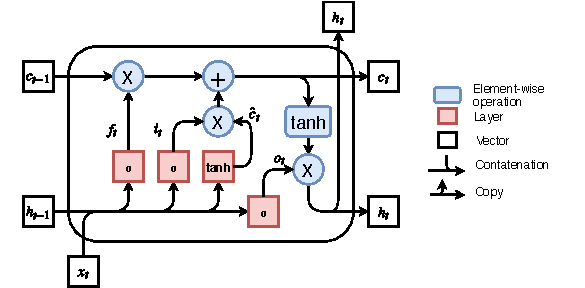
\includegraphics[width=.5\textwidth]{images/LSTM_cell.pdf}
		\label{fig:LSTM_cell}}
	%\vfil
	\quad\quad
	\subfigure[Multi-layer long short-term memory cell configuration.]{
		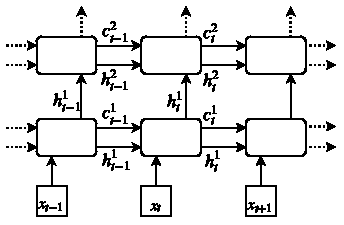
\includegraphics[width=.35\textwidth]{images/LSTM_multilayer.pdf}
		\label{fig:LSTM_multilayer}}
	\caption{An LSTM cell and it's multi-layer configuration in an RNN.}
	\label{fig:LSTM}
\end{figure}

First, data is removed from the cell state ($\vc$) as it flows through the LSTM cell.
The sigmoid function that produces $\vf_t$ outputs values between 0 and 1.
When these are multiplied with $\vc_{t-1}$ (the previous cell state) some elements will be removed or reduced.
The sigmoid layer that produces $\vf_t$ is referred to as the forget gate, as it causes some data to be ``forgotten" from the cell state depending on the previous cell output ($\vh_{t-1}$) and the current input ($\vx_t$).

Next, information is added to the cell state.
The tanh layer produces a new candidate cell state ($\hat{\vc}_t$), and the input gate layer produces $\vi_t$ in a similar fashion to $\vf_t$.
$\vi_t$ decides which elements of the new candidate cell state vector are added to the actual cell state vector by reducing the magnitude of elements in $\hat{\vc}_t$ based on the previous cell output ($\vh_{t-1}$) and the current input ($\vx_t$).
After $\hat{\vc}_t$ has been multiplied by $\vi_t$ to selectively reduce elements it is added to the cell state.
The sigmoid layer that produces $\vi_t$ is referred to as the input gate, as it decides what data is added to the cell state as it passes through the cell.

Finally, a candidate output vector is produced by applying tanh element-wise to the cell state.
The output gate layer produces $\vo_t$ and this is multiplied with the candidate output vector to selectively remove elements, producing the final cell output $\vh_t$.
The sigmoid layer that produces $\vo_t$ is referred to as the output gate, as it decides which elements of the candidate output are passed as the final output.

Together, these gating mechanisms allow the LSTM cell to selectively add and remove elements from the state as it passes through the cell, and allow the cell to selectively produce an output based on the cell state.
This allows the LSTM cell to retain data from many timesteps in the past, making it an appropriate choice when working with long sequences of data.

\subsection{Sequence to sequence recurrent neural network}
\label{section-S2S}
An RNN can be extended to form a sequence to sequence (S2S) architecture by applying an encoder RNN to an input sequence, and then having a decoder RNN produce an output sequence.
The decoder RNN's initial cell state is set to the final cell state of the encoder \cite{Cho2014a}.
This shared cell state is a latent representation of the input, which is used by the decoder to produce an output.
The encoder and decoder can be of different lengths, depicted in figure \ref{fig:S2S} as $R$ and $P$, allowing this architecture to naturally model tasks such as load forecasting where the input may be 48 hours of data while the output is only 24.
The output matrix $\mH \in \mathbb{R}^{R \times d}$ is then projected to the desired dimension.

Of course, an immediately obvious issue with this model is whether the shared latent cell state vector is capable of representing the input information in its entirety.

\begin{figure}[htbp]
	\centerline{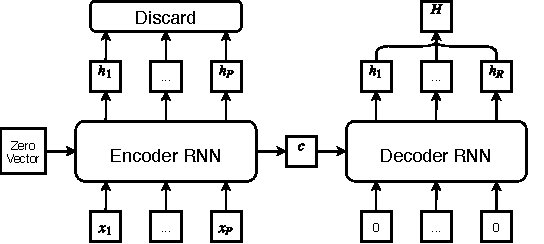
\includegraphics[trim=0 0cm 0 0, width=.75\textwidth]{images/S2S.pdf}}
	\caption{A sequence to sequence recurrent neural network architecture.}
	\label{fig:S2S}
\end{figure}

\subsection{Implementation}
A S2S RNN with LSTM cells was implemented in tensorflow \cite{tensorflow2015-whitepaper}, building on an implementation by \citet{Chevalier2017}.
The encoder was provided with historical load and weather, and forecast weather.
The projected decoder output was used as the load forecast.

The input vectors, $\vx_i$, are from the input matrix $\mX \in \mathbb{R}^{T \times N}$, where $\vx_i = (\mX_{i,:})^\top$, $T$ is the sequence length of the time series input, and $N$ is the number of observations at each point in the time series.

The decoder output, $\mH \in \mathbb{R}^{U \times d}$, was projected to a dimension of 1 using equation \ref{dense_layer}, where $\boldsymbol{W} \in \mathbb{R}^{d \times 1}$ is a learned weight matrix and $\boldsymbol{b} \in \mathbb{R}^{1}$ is a learned bias vector, $U$ is the length of the time series forecast, and $d$ is the hidden dimension of the model.

\section{Transformer} \label{sec:transformer}
The transformer neural network architecture, shown in figure \ref{fig:transformer}, was introduced by \citet{Vaswani2017} in 2017 and at the time was the state of the art in neural machine translation.
It has since been outperformed by a variant of itself, the universal transformer \cite{Dehghani2018}, which is discussed in section \ref{sec:universal_transformer}.
A transformer-based neural network has been applied to time series classification and regression in a medical context, achieving state of the art results \cite{Song2017}.
The transformer has been extended to the image transformer model, which achieves state of the art results in image generation tasks \cite{Parmar2018}.
To the best of the author's knowledge, there are no publications which apply the transformer -- or any similar architecture -- to electrical load forecasting.

The transformer architecture follows a similar sequence-to-sequence/encoder-decoder architecture as the sequence to sequence RNN architecture described in section \ref{section-S2S}: the encoder transforms an input sequence $\mX = [\vx_1 \, \ldots \, \vx_P]$ into a latent representation $\mZ = [\vz_1 \, \ldots \, \vz_M]$, and the decoder transforms $\mZ$ into an output sequence $\mY = [\vy_1 \, \ldots \, \vy_R]$.
This aligns with the requirements of a load forecasting system, where $P$ is the length of the time series input, $\vx_t$ is of dimension equal to the number of variables in the input time series, $R$ is the length of the time series output, and $\vy_t$ is of dimension equal to the number of variables in the output time series.
The latent representation $\mZ$ is used solely by the model as an internal representation of the input data.

\begin{figure}[htbp]
	\centerline{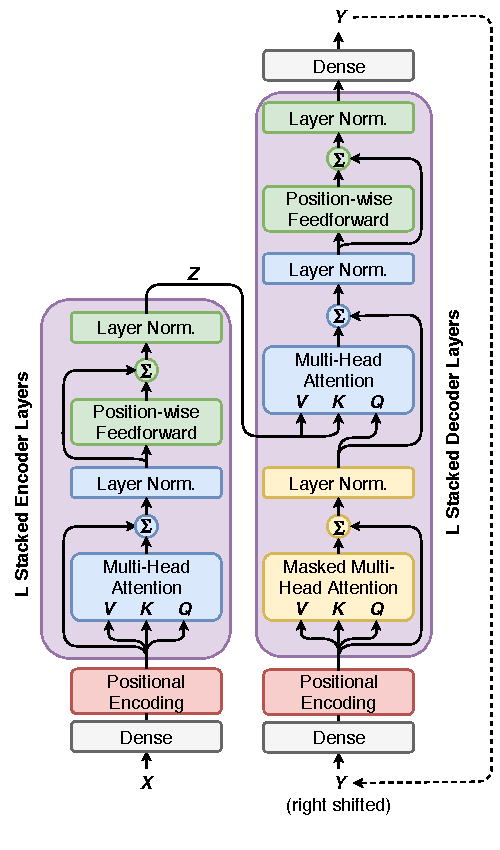
\includegraphics[trim=0 0cm 0 0, width=.4\textwidth]{images/transformer.pdf}}
	\caption{The Transformer architecture.}
	\label{fig:transformer}
\end{figure}

The encoder is constructed of a stack of $L$ identical layers, each containing two sub-layers.
The first is multi-head self-attention and the second is a position-wise feed-foward network.
Both sub-layers have a residual connection around them and are fed into a normalization layer.

The decoder is similar to the encoder except for a third layer which implements multi-head attention on the final output of the encoder.
The input to the decoder is the output of the decoder, but shifted right by one.
This requires an iterative approach to be used to predict all points in the time series.
The self-attention in the decoder is masked so that when evaluating a query at time $t$ it does not assign large weights to keys/values occurring after $t$ in time, making the decoder autoregressive.

The individual components of the transformer are discussed in the following sections.

\subsection{Input Embedding}
The input $\boldsymbol{X} \in \mathbb{R}^{T \times N}$, where the rows represent $T$ points in time and the columns represent $N$ time series, is embedded by applying a dense layer to produce an embedded $\boldsymbol{X'} \in \mathbb{R}^{T \times d}$, where $d$ is the hidden dimension of the model and $d$ is the same for both the encoder and the decoder.
This is intended to allow the neural network to learn the relationships and dependencies between the different input time series.
The embedded representation is given by Equation \ref{dense_layer}, with learned weights $\boldsymbol{W} \in \mathbb{R}^{N \times d}$ and a learned bias vector $\boldsymbol{b} \in \mathbb{R}^{d}$.

\begin{equation} \label{dense_layer}
\text{dense}(\boldsymbol{X}) = \text{max}(0, \boldsymbol{XW} + \boldsymbol{b})
\end{equation}

\subsection{Positional Encoding} \label{sec:positional_encoding}
The model has no way of telling the position or order of each element in the input, so this information is injected in the positional encoding layer.
This is done by using a learned lookup table to add the same value to the inputs at both test and train time depending on their position in time in the input.
Specifically, the positional encoding layer adds a matrix lookup table of embeddings $\boldsymbol{E}$ to the input, where $\boldsymbol{E}$ is of the same dimension as the input.

\subsection{Multi-Head Attention} \label{multihead_attention}
The primary innovation of the Transformer architecture is multi-head attention.
Generic attention and dot-product attention will now be described as these are prerequisite to describing multi-head attention.

Given a single query vector and a set of key and value pairs (with each key and each value being a vector), an attention function matches the query to the keys to produce a weight for each key by applying an arbitrary fitness function.
These key weights are then used to create an output vector comprised of the weighted sum of the values, where each value's weight is the weight assigned to its corresponding key. 

\begin{figure}[htbp]
	\centerline{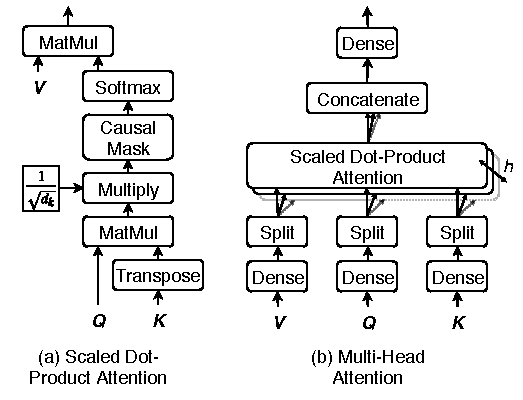
\includegraphics[width=.35\textwidth]{images/multihead_attn.pdf}}
	\caption{Multiheaded attention (b) splits the key, query, and value matrices and applies scaled dot product attention (a) on each in parallel before concatenating the result to return the data to its original dimension.}
	\label{fig:multihead}
\end{figure}

Scaled dot-product attention, shown in Figure \ref{fig:multihead} (a), is a specific implementation of an attention function. 
It uses the dot product of the query and each key to generate the weights, which are then passed through a softmax function such that the sum of all weights is equal to 1.
In practice, the query row vectors are combined into a single matrix, $\boldsymbol{Q}$, allowing cheap matrix calculations to be used to evaluate the attention outputs in parallel.
The keys and values are represented by row vectors in $\boldsymbol{K}$ and $\boldsymbol{V}$, respectively.

The dot product of the keys and queries is scaled (hence the name) by multiplying it by $1 / \sqrt{d_k}$, with $d_k$ being the key and query dimension, to prevent the dot product from becoming large when $d_k$ is large as this may cause the softmax gradient to become very small and affect the gradient descent training.

The causal mask shown in Figure \ref{fig:multihead} is used exclusively in the decoder self-attention to prevent the attention function from matching any query to a key that occurs after itself in time.
This is achieved by leaving the lower triangular portion of the matrix untouched and setting the other values to be large negative numbers, indicating a very poor match.

Multi-head attention, shown in Figure \ref{fig:multihead} (b), applies a separate dense layer to each of the values, queries, and keys. 
The dense layer is applied per Equation \ref{dense_layer} with learned weights $\boldsymbol{W} \in \mathbb{R}^{d \times d}$ and a learned bias vector $\boldsymbol{b} \in \mathbb{R}^{d}$.
The outputs of the dense layers are then split along the last axis into $h$ sets, or heads.
As a result the key, query, and value dimension is reduced by a factor of $h$ to $\frac{d}{h}$.
Scaled dot-product attention is then run independently on each set.
The results are concatenated and put through a final dense layer to produce the output of the attention function.
The dense layer function on the output is defined by Equation \ref{dense_layer} where $\boldsymbol{W} \in \mathbb{R}^{d \times d}$ is a learned weight matrix and $\boldsymbol{b} \in \mathbb{R}^{d}$ is a learned bias vector.

The dense layer combined with the split allows the multi-head attention to pick out information from different subspaces in the input and direct these to different attention heads.
This is in contrast to a single head which must average all subspaces.

\subsection{Feed-forward}
The feed-forward layer is a two layer network with a rectified linear unit in the middle.
Given an input $\boldsymbol{X} \in \mathbb{R}^{T \times d}$, the output $\boldsymbol{X'} \in \mathbb{R}^{T \times d}$ is populated by Equation \ref{feedforward} where $\boldsymbol{W}_1 \in \mathbb{R}^{d \times 4d}$, $\boldsymbol{b}_1 \in \mathbb{R}^{4d}$, $\boldsymbol{W}_2 \in \mathbb{R}^{4d \times d}$, and $\boldsymbol{b}_2 \in \mathbb{R}^{d}$ are learned weights and biases.

\begin{equation} \label{feedforward}
\text{feedforward}(\boldsymbol{X}) = \text{max}(0, \boldsymbol{X}  \boldsymbol{W}_1 + \boldsymbol{b}_1)  \boldsymbol{W}_2 + \boldsymbol{b}_2
\end{equation}

\subsection{Decoder Dense Output}
The output of the decoder is passed through a dense layer to project the hidden dimension to the desired dimension of 1.
The layer is implemented per Equation \ref{dense_layer} where $\boldsymbol{W} \in \mathbb{R}^{d \times 1}$ is a learned weight matrix and $\boldsymbol{b} \in \mathbb{R}^{1}$ is a learned bias vector.
By adjusting the dimension of $\boldsymbol{W}$ and $\boldsymbol{b}$ the network could be modified to perform multiple forecasts simultaneously.


\subsection{Residuals \& Normalization}
Residual connections \cite{He2015} are applied around each sub-layer.
That is, the output of each sub-layer is given by $\boldsymbol{X'} = \boldsymbol{X} + \text{subLayer}(\boldsymbol{X})$ where subLayer$(\boldsymbol{X})$ is the original output of the sub-layer.
The outputs are then normalized by applying layer normalization \cite{Ba2016}.

\subsection{Dropout and Training}
To help prevent overfitting to the training data, dropout \cite{srivastava14a} is applied during training at the output of both positional encoding layers, and immediately after the softmax operation in all multi-head attention layers.

When testing or being used for inference, the decoder outputs are generated sequentially one at a time.
After each output value is generated it is shifted right by one and populated in the decoder input and the model is executed again until all the outputs have been generated.
Values that have not yet been generated are set to zero in the decoder input.
These zero values do not affect the output of the decoder, as the decoder self-attention is masked so that it does not make use of them.
When training, the decoder input is set to the known expected value and the model is executed --- and the learnable parameters updated --- a single time.

This process of supplying the known good values - or the previously generated values when in inference mode - to the decoder input is known as teacher forcing or professor forcing \cite{lamb2016professor}.
This is common practice in neural machine translation (NMT), but does not necessarily make sense in time series forecasting tasks.
In NMT, words are usually represented as vectors with hundreds or thousands of elements.
Adjacent words in the sentences are nearly always very different.
However, in time series forecasting, the input vectors adjacent to each other are very similar.
That is, the time series data generally has a high autocorrelation - for example the time series at 12pm and 1pm are likely to be very similar.
This results in the model tending to simply reproduce the input at the output, as this results in a time series forecast that is perfect except shifted forward in time by one period.

This effect was overwhelming in the sequence to sequence models and caused the models to fail to converge, and so teacher forcing was never used.
In the transformer, on the other hand, the models still converged.
However, the performance of the models with and without teacher forcing is different.

\subsection{Implementation}
The encoder was provided with historical load and weather, and forecast weather.
The decoder output was projected to a dimension of 1 and taken as the load forecast.

\section{Universal Transformer} \label{sec:universal_transformer}
The universal transformer, shown in figure \ref{fig:universal_transformer}, is a variation on the transformer where the layers within the encoder and decoder (except for the timestep encoding) share parameters.
This architecture was published in July 2018 \cite{Dehghani2018} and there are only two published publications which reference it.
The universal transformer outperforms the original transformer in the following tasks \cite{Dehghani2018}:
\begin{itemize}
	\item Neural machine translation -- at which the universal transformer is the state of the art.
	\item Algorithmic tasks: copying the input to the output, copying the reversed input to the output, and adding values from the input.
	\item Natural language question-answering.
	\item Natural language modelling.
\end{itemize}

\begin{figure}[htbp]
	\centerline{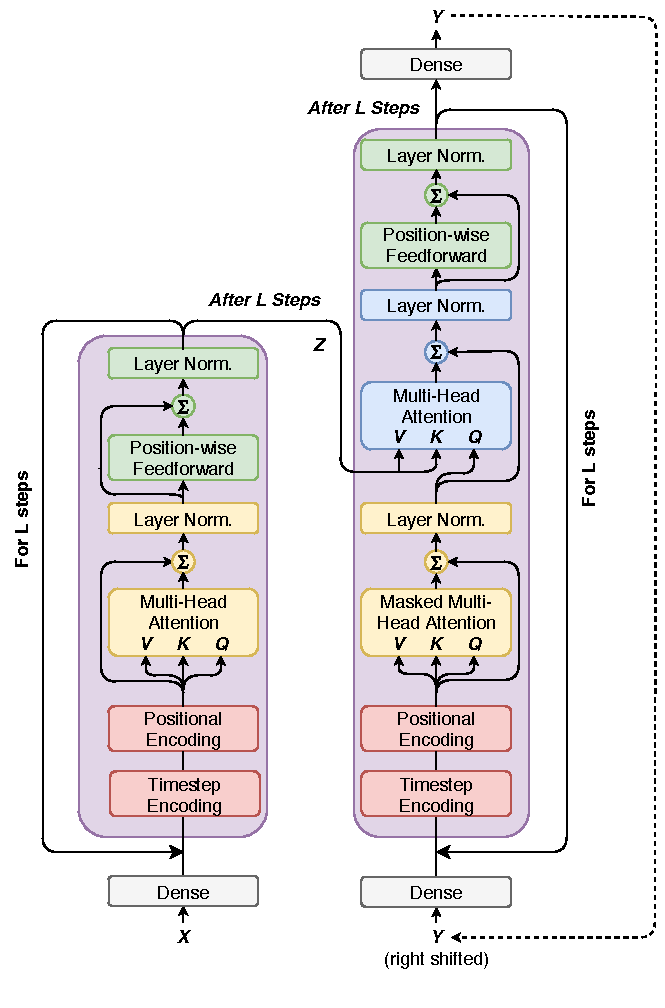
\includegraphics[width=.5\textwidth]{images/universal_transformer.pdf}}
	\caption{Universal transformer architecture.}
	\label{fig:universal_transformer}
\end{figure}

All layers within the encoder and decoder layers of the universal transformer are identical to those described in section \ref{sec:transformer}.
In the universal transformer, the encoder and decoder are stacked $L$ times just as they are in the transformer.
However in the universal transformer, all of the weights within the encoder layers are shared, and all the weights within the decoder layers are shared.
This results in the depiction shown in figure \ref{fig:universal_transformer}, where the output of each encoder/decoder layer is fed back into itself $L$ times.

The exception to this weight sharing is the temporal encoding layer.
This layer is identical to the positional encoding layer described in section \ref{sec:positional_encoding} and allows the model to keep track of which point in time (how many times it has recurred so far) it is currently at.

The original universal transformer publication specifies sinusoidal positional and timestep encoding \cite{Dehghani2018}.
The use of sinusoidal encoding versus fixed learned encoding (as used in this thesis) is discussed in the paper that originally presents the transformer \cite{Vaswani2017}, with the conclusion that it produces nearly identical results to sinusoidal encoding.
The authors note in \cite{Vaswani2017} that sinusoidal encoding is preferable in neural machine translation applications (where sequence lengths are variable and dictated by sentence lengths) because it allows the model to generalize to sequence lengths that it has not encountered during training.
In the applications in this thesis, all sequence lengths are constant.
For this reason, fixed learned encoding is used in the universal transformer in this thesis.
One downside to using fixed learned encoding is that it introduces more parameters to the model, which may have negative effects on the performance and training of the model.


\subsection{Implementation}
The encoder was provided with historical load and weather, and forecast weather.
The decoder output was projected to a dimension of 1 and taken as the load forecast.


\section{Training and regularization of neural networks}
\label{train-reg}
Training and regularization is common to all described neural network models.
The encoder inputs, decoder inputs, and expected outputs were summed with randomly distributed noise with a mean of 0 and standard deviation of 0.01 before being supplied to the model during training.
This has been demonstrated to improve the generalization ability of a neural network \cite{Wang1999} \cite{Brown2003} and can be considered an extension of dropout \cite{srivastava14a}.

All models were trained using the Adam optimizer \cite{Kingma2014} and a modified sum of errors squared loss function.
Given a vector $\boldsymbol{\hat{y}}$ of predictions from the model and a vector $\boldsymbol{y}$ of expected predictions the loss function $l$ is given by 
\begin{equation}
l = \sum_{t=0}^{R}((\boldsymbol{y}_t - \boldsymbol{\hat{y}}_t)^2 \times |\boldsymbol{y}_t|^c)
\end{equation}
where $c$ is a model hyperparameter.
For $c>0$ this function accentuates loss when the actual value is large --- making the model more accurate at forecasting peaks.


\section{Similar profile selection} \label{simperiod}
Load profiles are influenced by exogenous data such as weather, day of the week, and holiday type \cite{Weron2006}.
A simple and intuitive method of load forecasting is to find periods in the past with similar exogenous data to the period being forecast and then use the load profiles from these past periods to form a forecast \cite{Senjyu1998}.
However, these similar period methods can be insufficient to capture complex patterns, especially over holiday periods which occur only once per year \cite{Chen2010}.

%Holiday type indicates which holiday the load profile occurs on - Easter or Christmas for example.
%These different holidays are assigned different integer identifiers (with normal days assigned identifier 0) to form a time series.

The forecasting system was provided with historical load and weather profiles from periods that had similar exogenous data to the period of the load profile being forecast.
Similar periods were identified by first finding candidate similar periods an integer multiple of 1 year $\pm$30 days away from the period being forecast.
These candidates were then filtered down to periods with exactly matching hour and minute.

Then the weighted Euclidean distance between the period being forecast and each candidate similar period was calculated using the following features: 
\begin{itemize}
	\item maximum future (forecast) temperature, 
	\item minimum future (forecast) temperature,
	\item maximum past load,
	\item current holiday type, 
	\item current day of the week,
	\item current day of the month, and
	\item current month of the year.
\end{itemize}

The holiday type indicates the current holiday --- Easter or Christmas for example --- and is encoded as a time series of integers with a different integer for each holiday.
When the holiday type always occurs on the same date each year then the month of the year and day of the month were used, whereas when the holiday type always occurs on the same day of the week each year then the day of the week was used.
The candidate similar periods with the lowest Euclidean distance were selected as the final set of similar periods.

When training and testing the model the similar periods were selected from both the past and the future, as the train and test datasets were only five years each.
It was assumed that, for testing, there were no changes in the patterns underlying the load profile over the duration of the testing set.